% Preamble additions (recommended)
% \usepackage{graphicx}
% \usepackage{subcaption}
% \usepackage{placeins}   % for \FloatBarrier
% \usepackage{float}      % if you want [H] placement (optional)

\section{Appendices}

\begin{appendices}

% ---------- A: GMM model tuning ----------
\clearpage                    % start this appendix section on a new page
\section{GMM model tuning}

Model tuning across all cohorts favored Gaussian mixtures with full covariance matrices, yielding lower Bayesian Information Criterion (BIC; lower is better) and higher average Bhattacharyya distances between components (greater separation). Performance improved up to \(K=8\) and then showed diminishing returns, so we fixed \(K=8\) for the main analyses. All principal findings were confirmed in a sensitivity analysis with \(K \in \{6,\ldots,11\}\).


\begin{figure}[p]
  \centering
  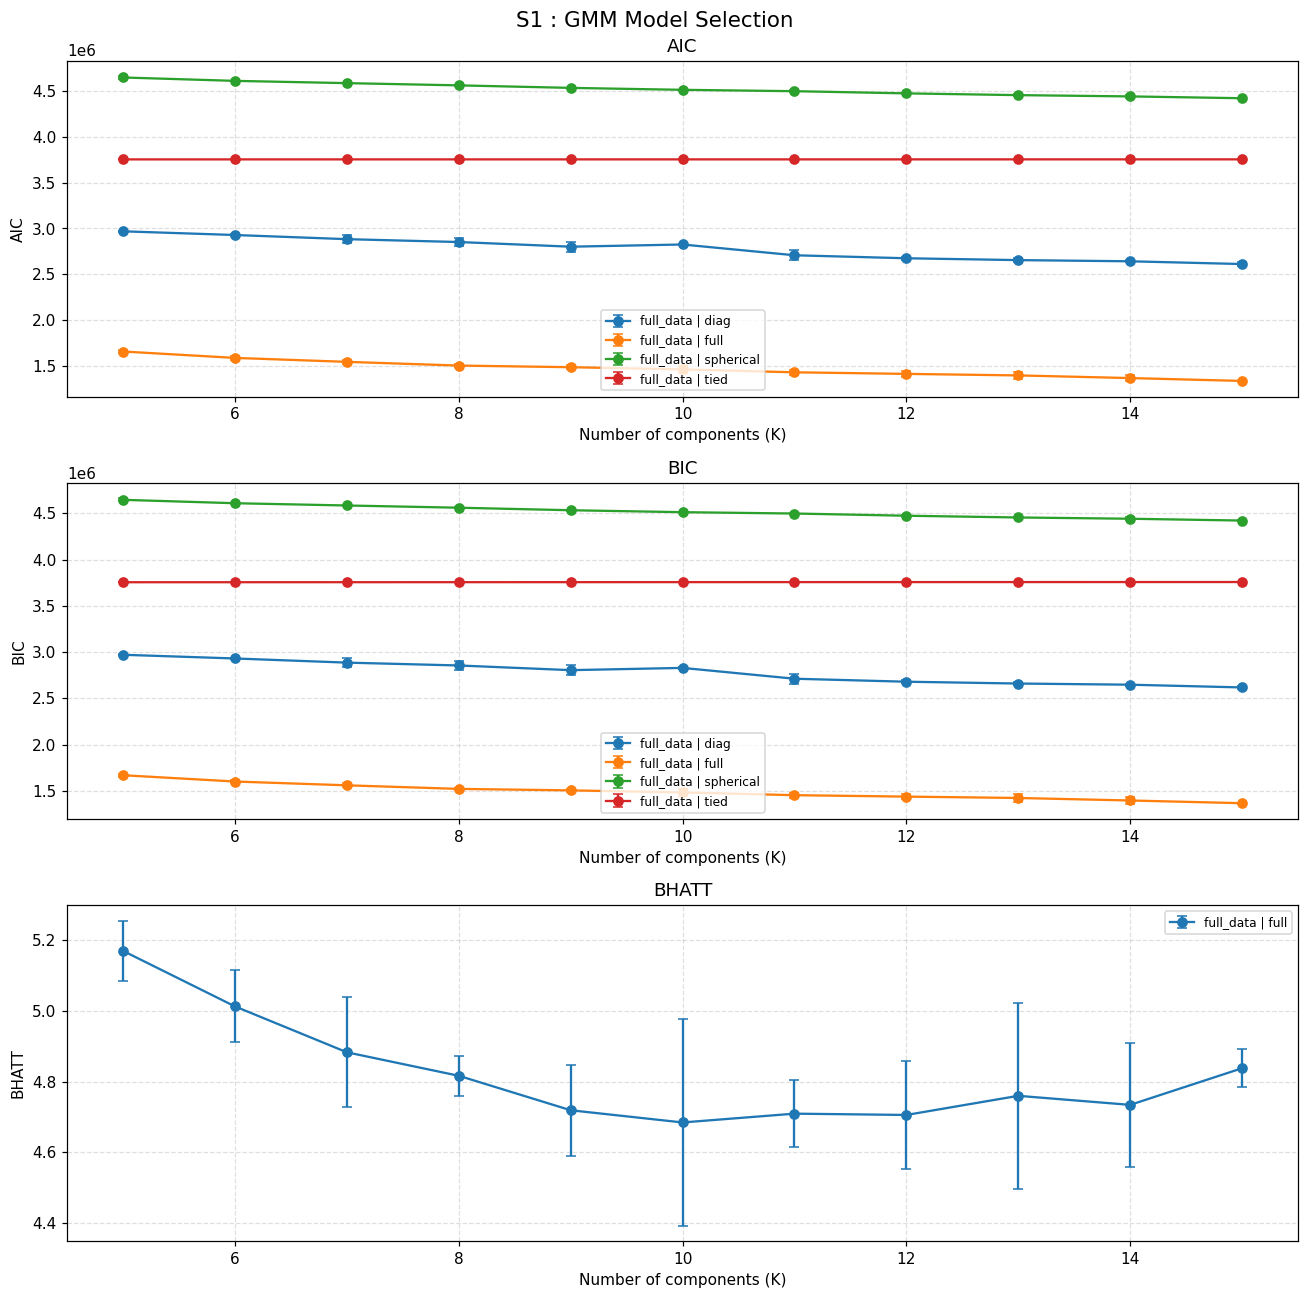
\includegraphics[width=\linewidth]{figures/appendix/tesserae_gmm_model_selection.png}
  \caption{Tesserae: Model selection}
  \label{fig:tesserae_model_selection}
\end{figure}

\begin{figure}[p]
  \centering
  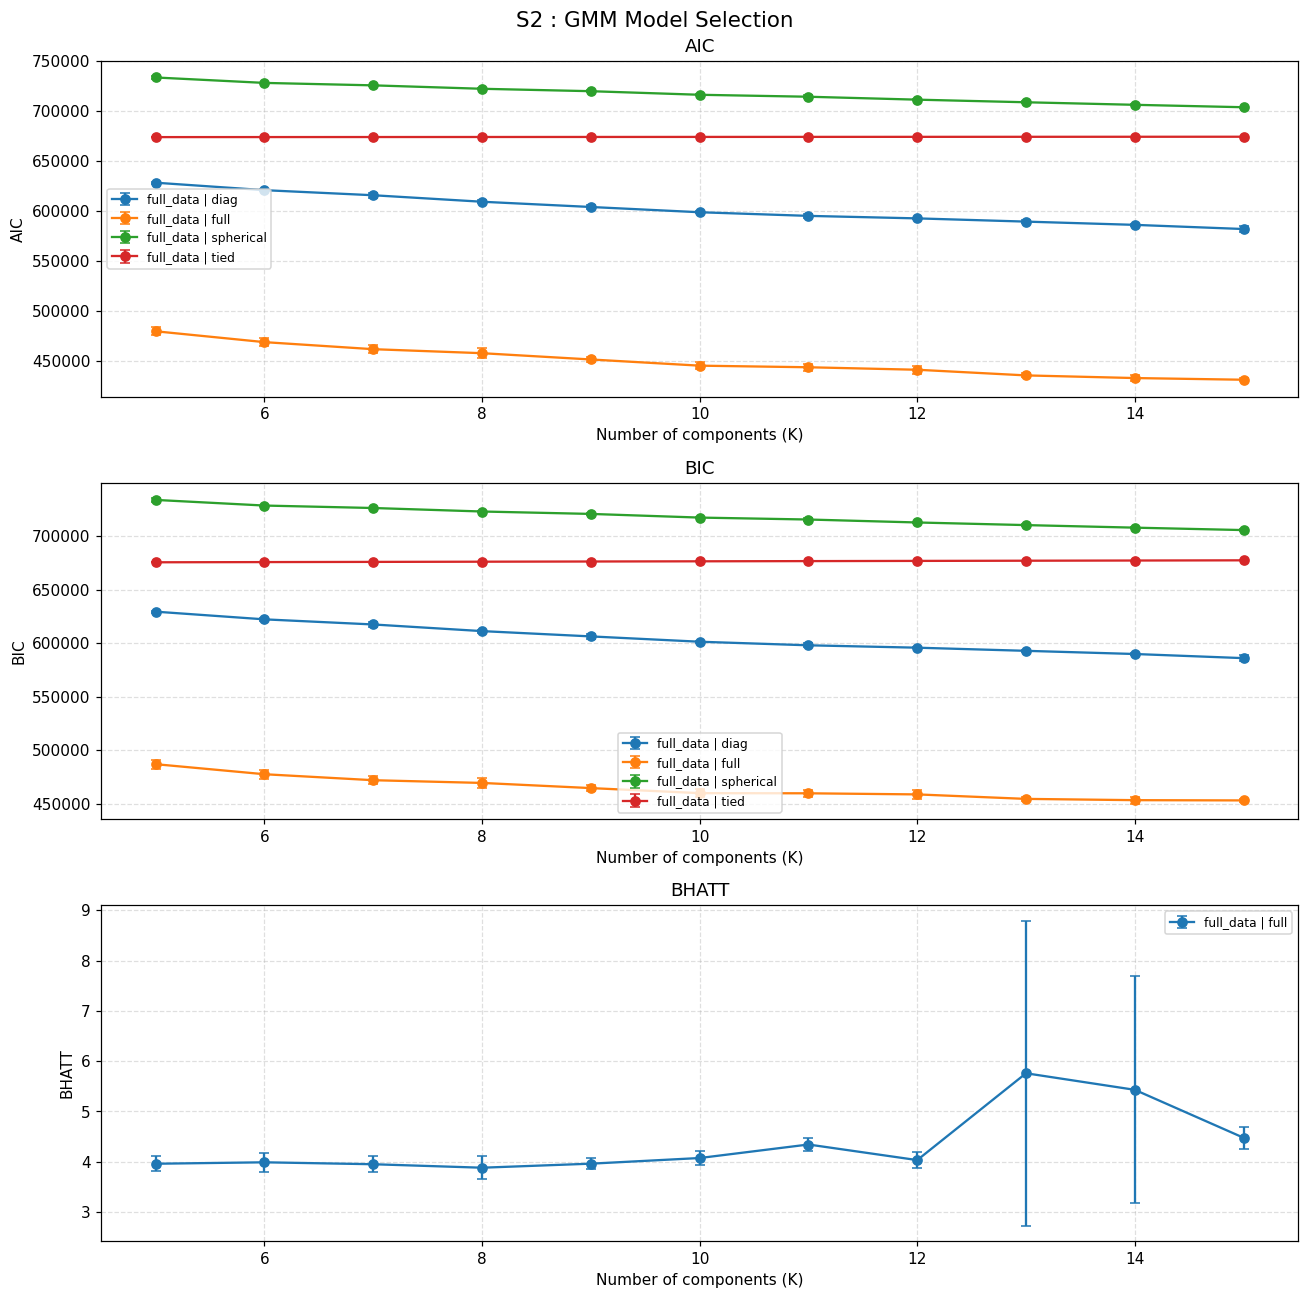
\includegraphics[width=\linewidth]{figures/appendix/momo_gmm_model_selection.png}
  \caption{MoMo-Mood: Model selection}
  \label{fig:momo_gmm_model_selection}
\end{figure}

\begin{figure}[p]
  \centering
  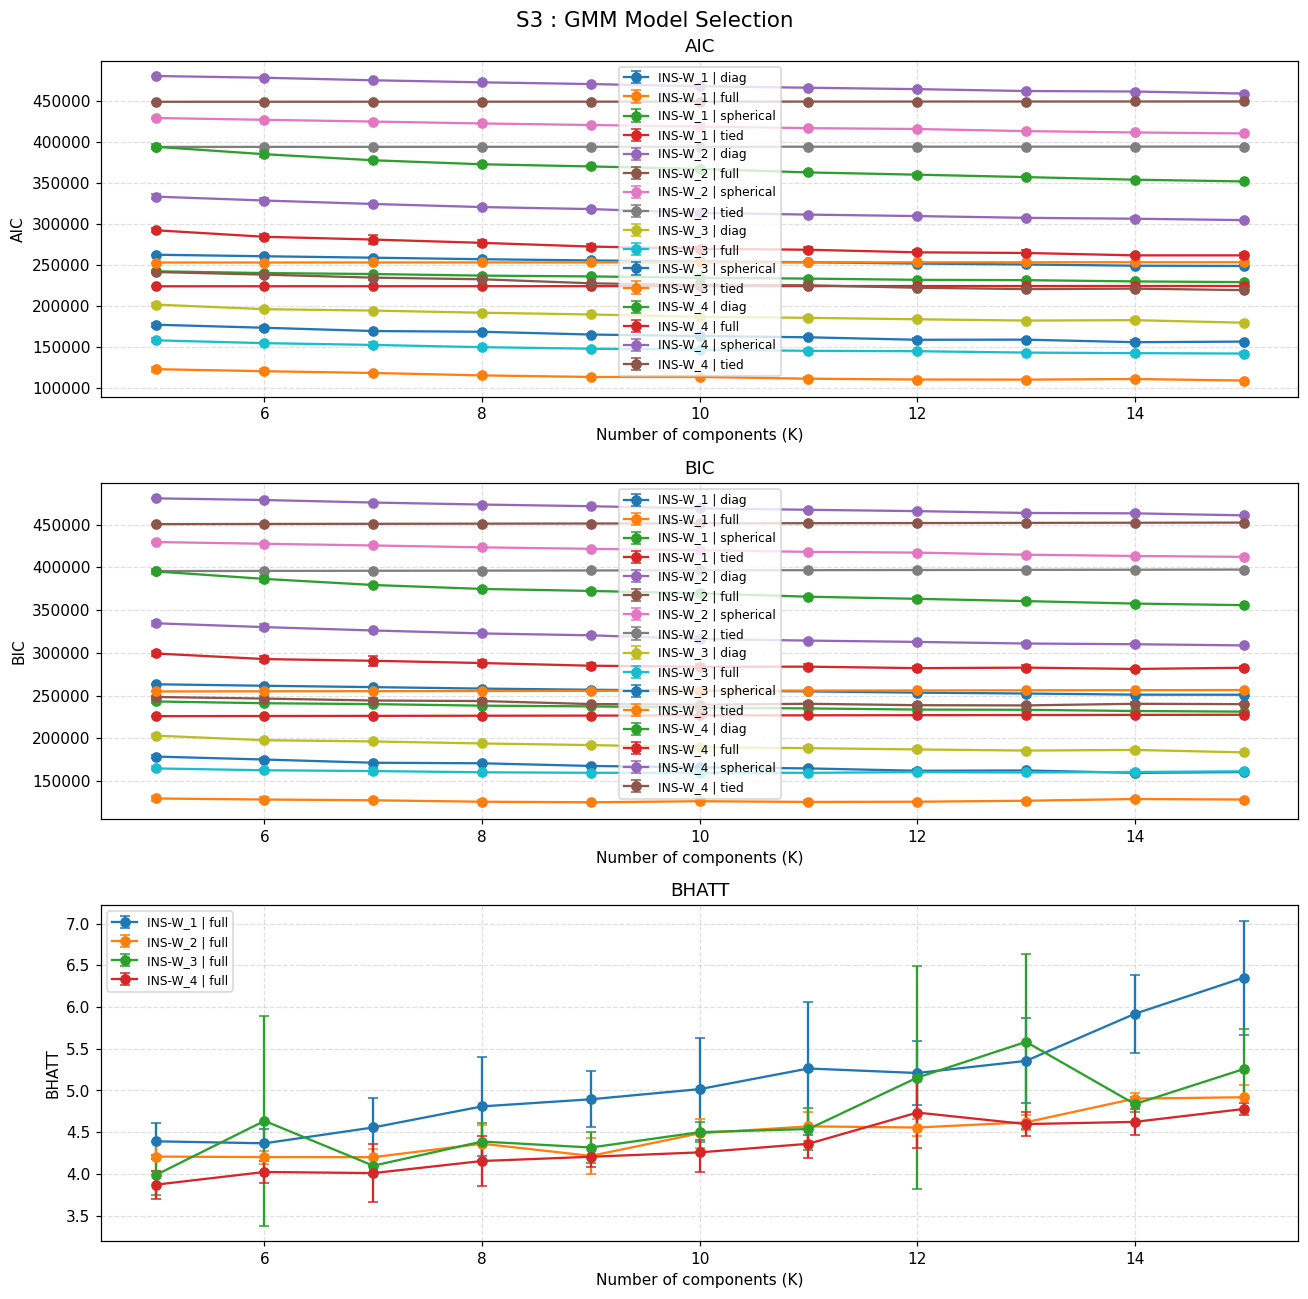
\includegraphics[width=\linewidth]{figures/appendix/globem_gmm_model_selection.png}
  \caption{GLOBEM: Model selection}
  \label{fig:globem_gmm_model_selection}
\end{figure}

\FloatBarrier                 % ensure these floats don’t spill into the next section

% ---------- B: Cluster properties ----------
\clearpage
\section{Cluster properties of MoMo-Mood and GLOBEM}

\autoref{fig:momo_centroid_summary} and \autoref{fig:globem_centroids} describe the cluster characteristics of the MoMo-Mood and GLOBEM studies, respectively. Across both datasets, a few dominant clusters account for the majority of time, while other clusters reflect free day routines, for example, elevated nightly activity or increased nighttime screen use.

\begin{figure}[p]
  \centering
  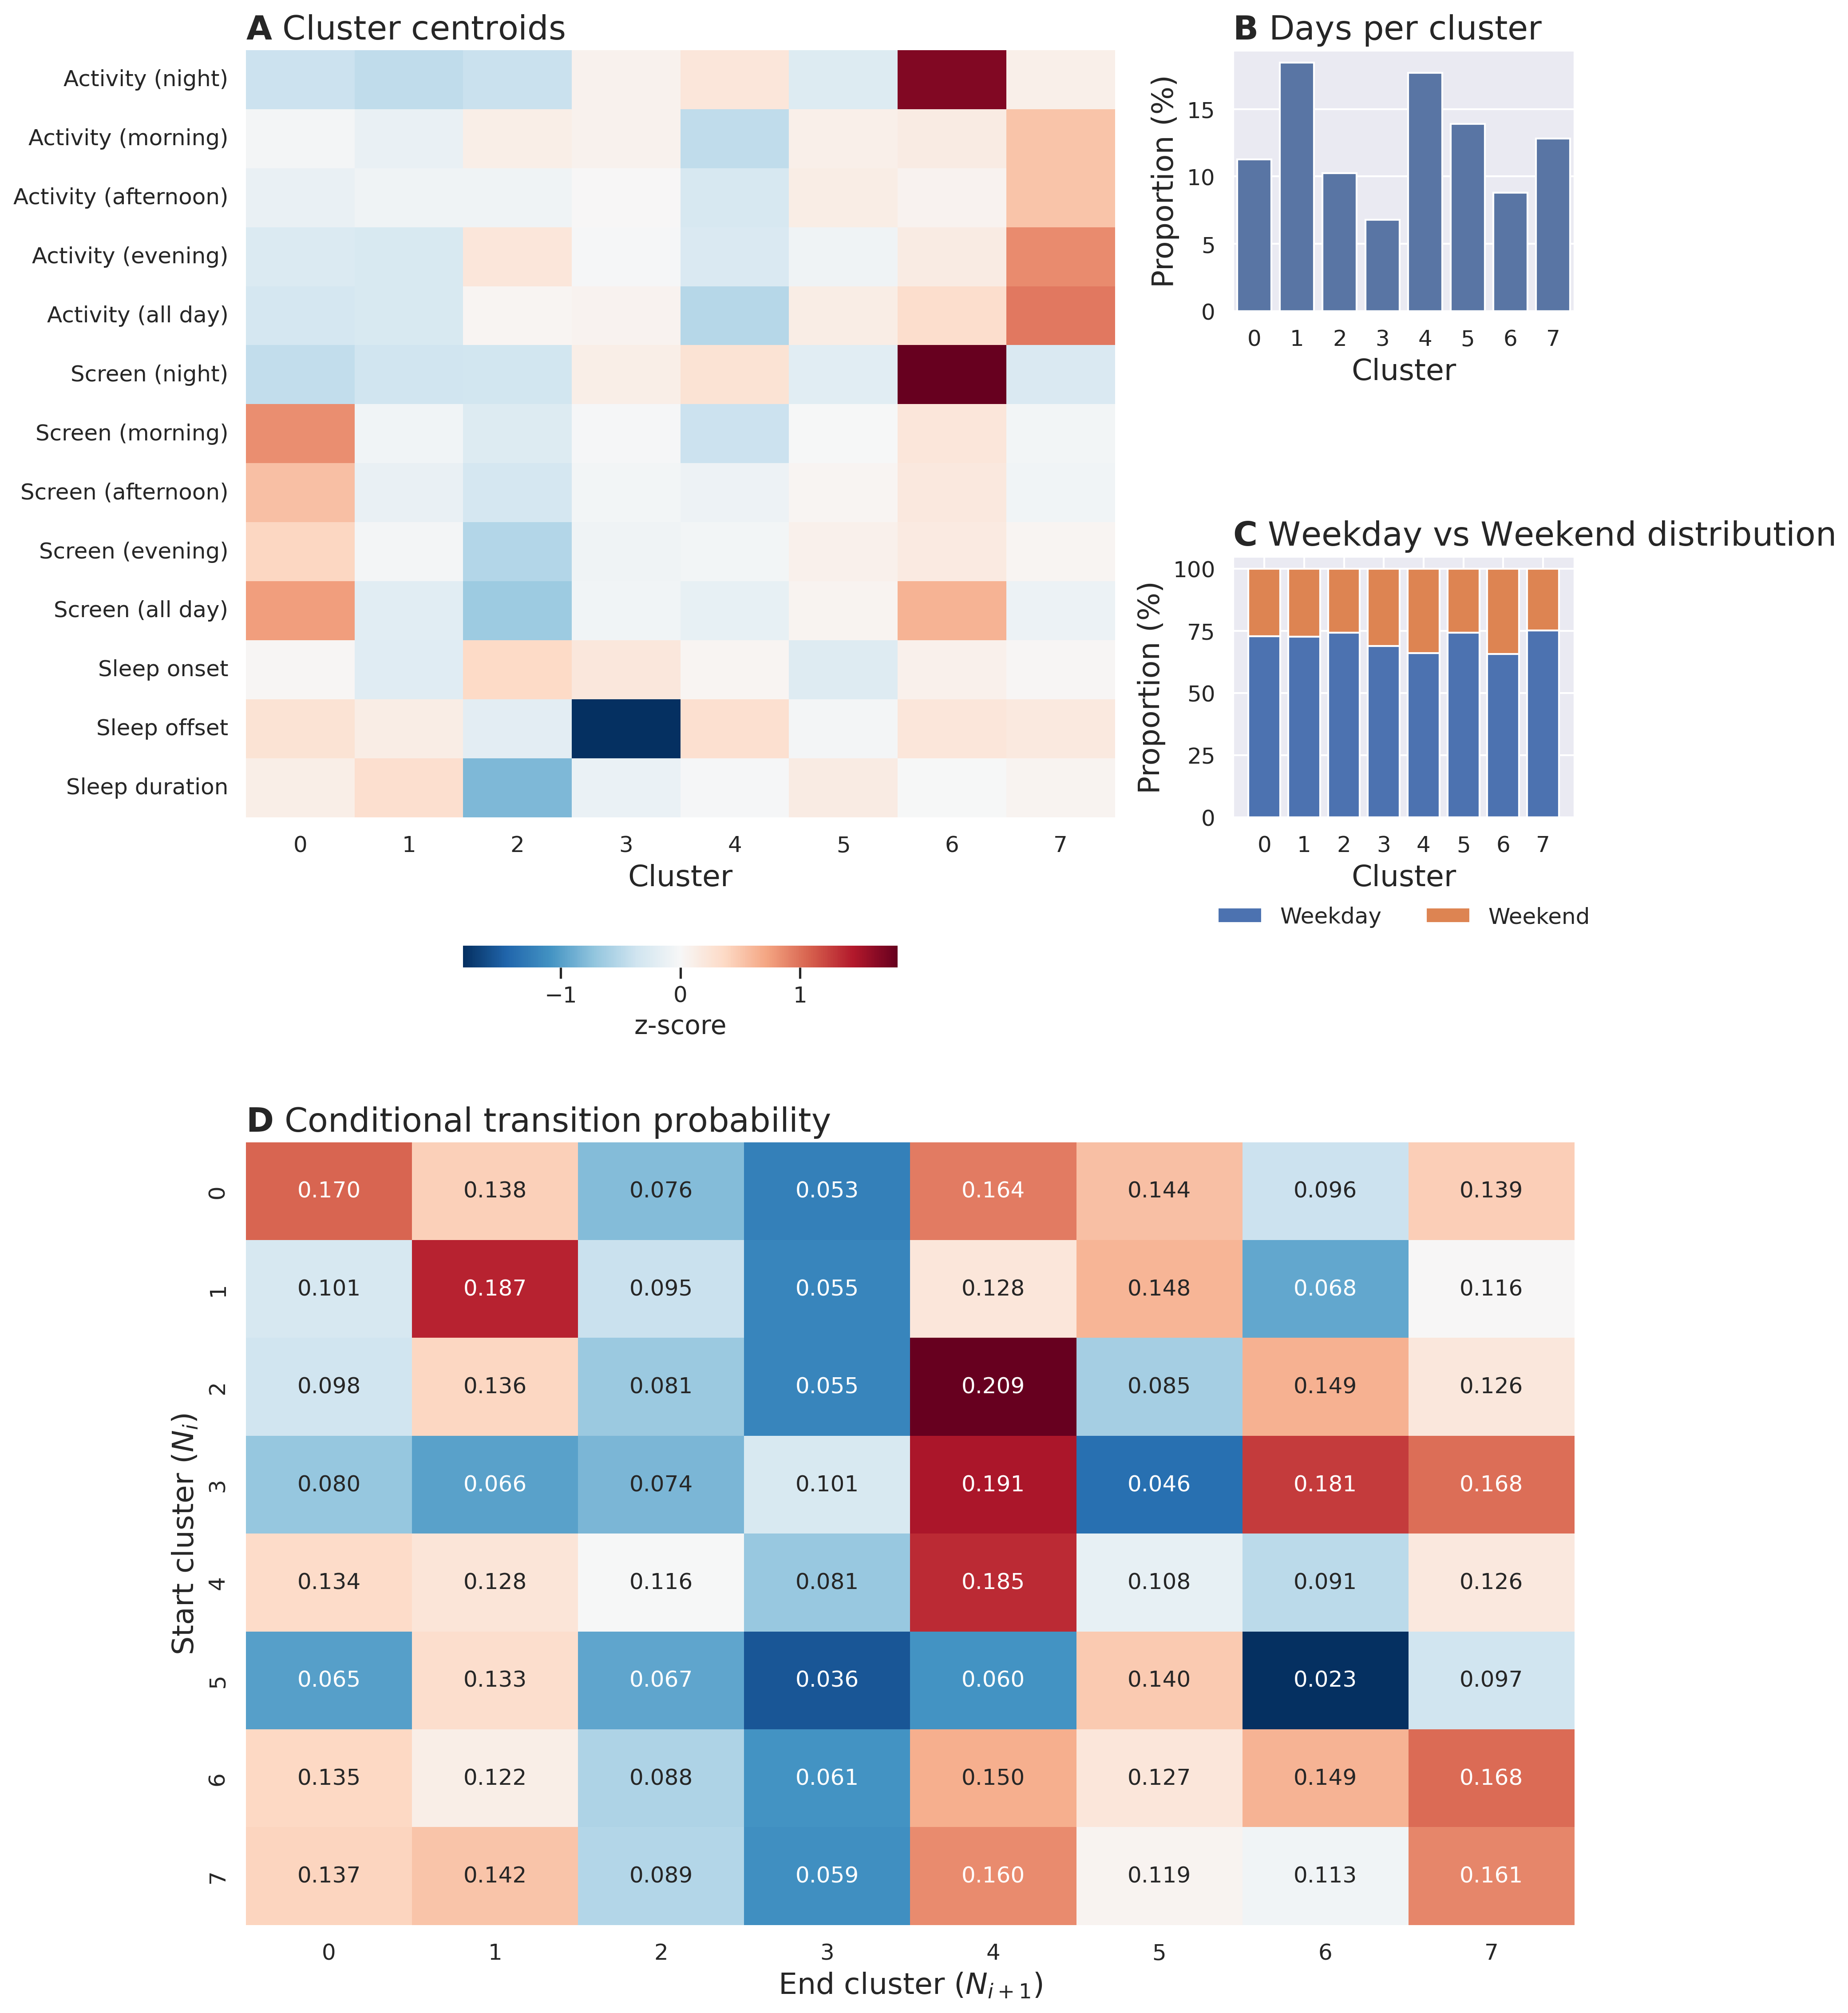
\includegraphics[width=\linewidth]{figures/appendix/momo_summary.png}
  \caption{MoMo-Mood: Cluster centroid characteristics}
  \label{fig:momo_centroid_summary}
\end{figure}

% 2x2 subfigures for GLOBEM centroid characteristics (example filenames 1–4)
\begin{figure}[p]
  \centering

  \begin{subfigure}[t]{0.485\textwidth}
    \centering
    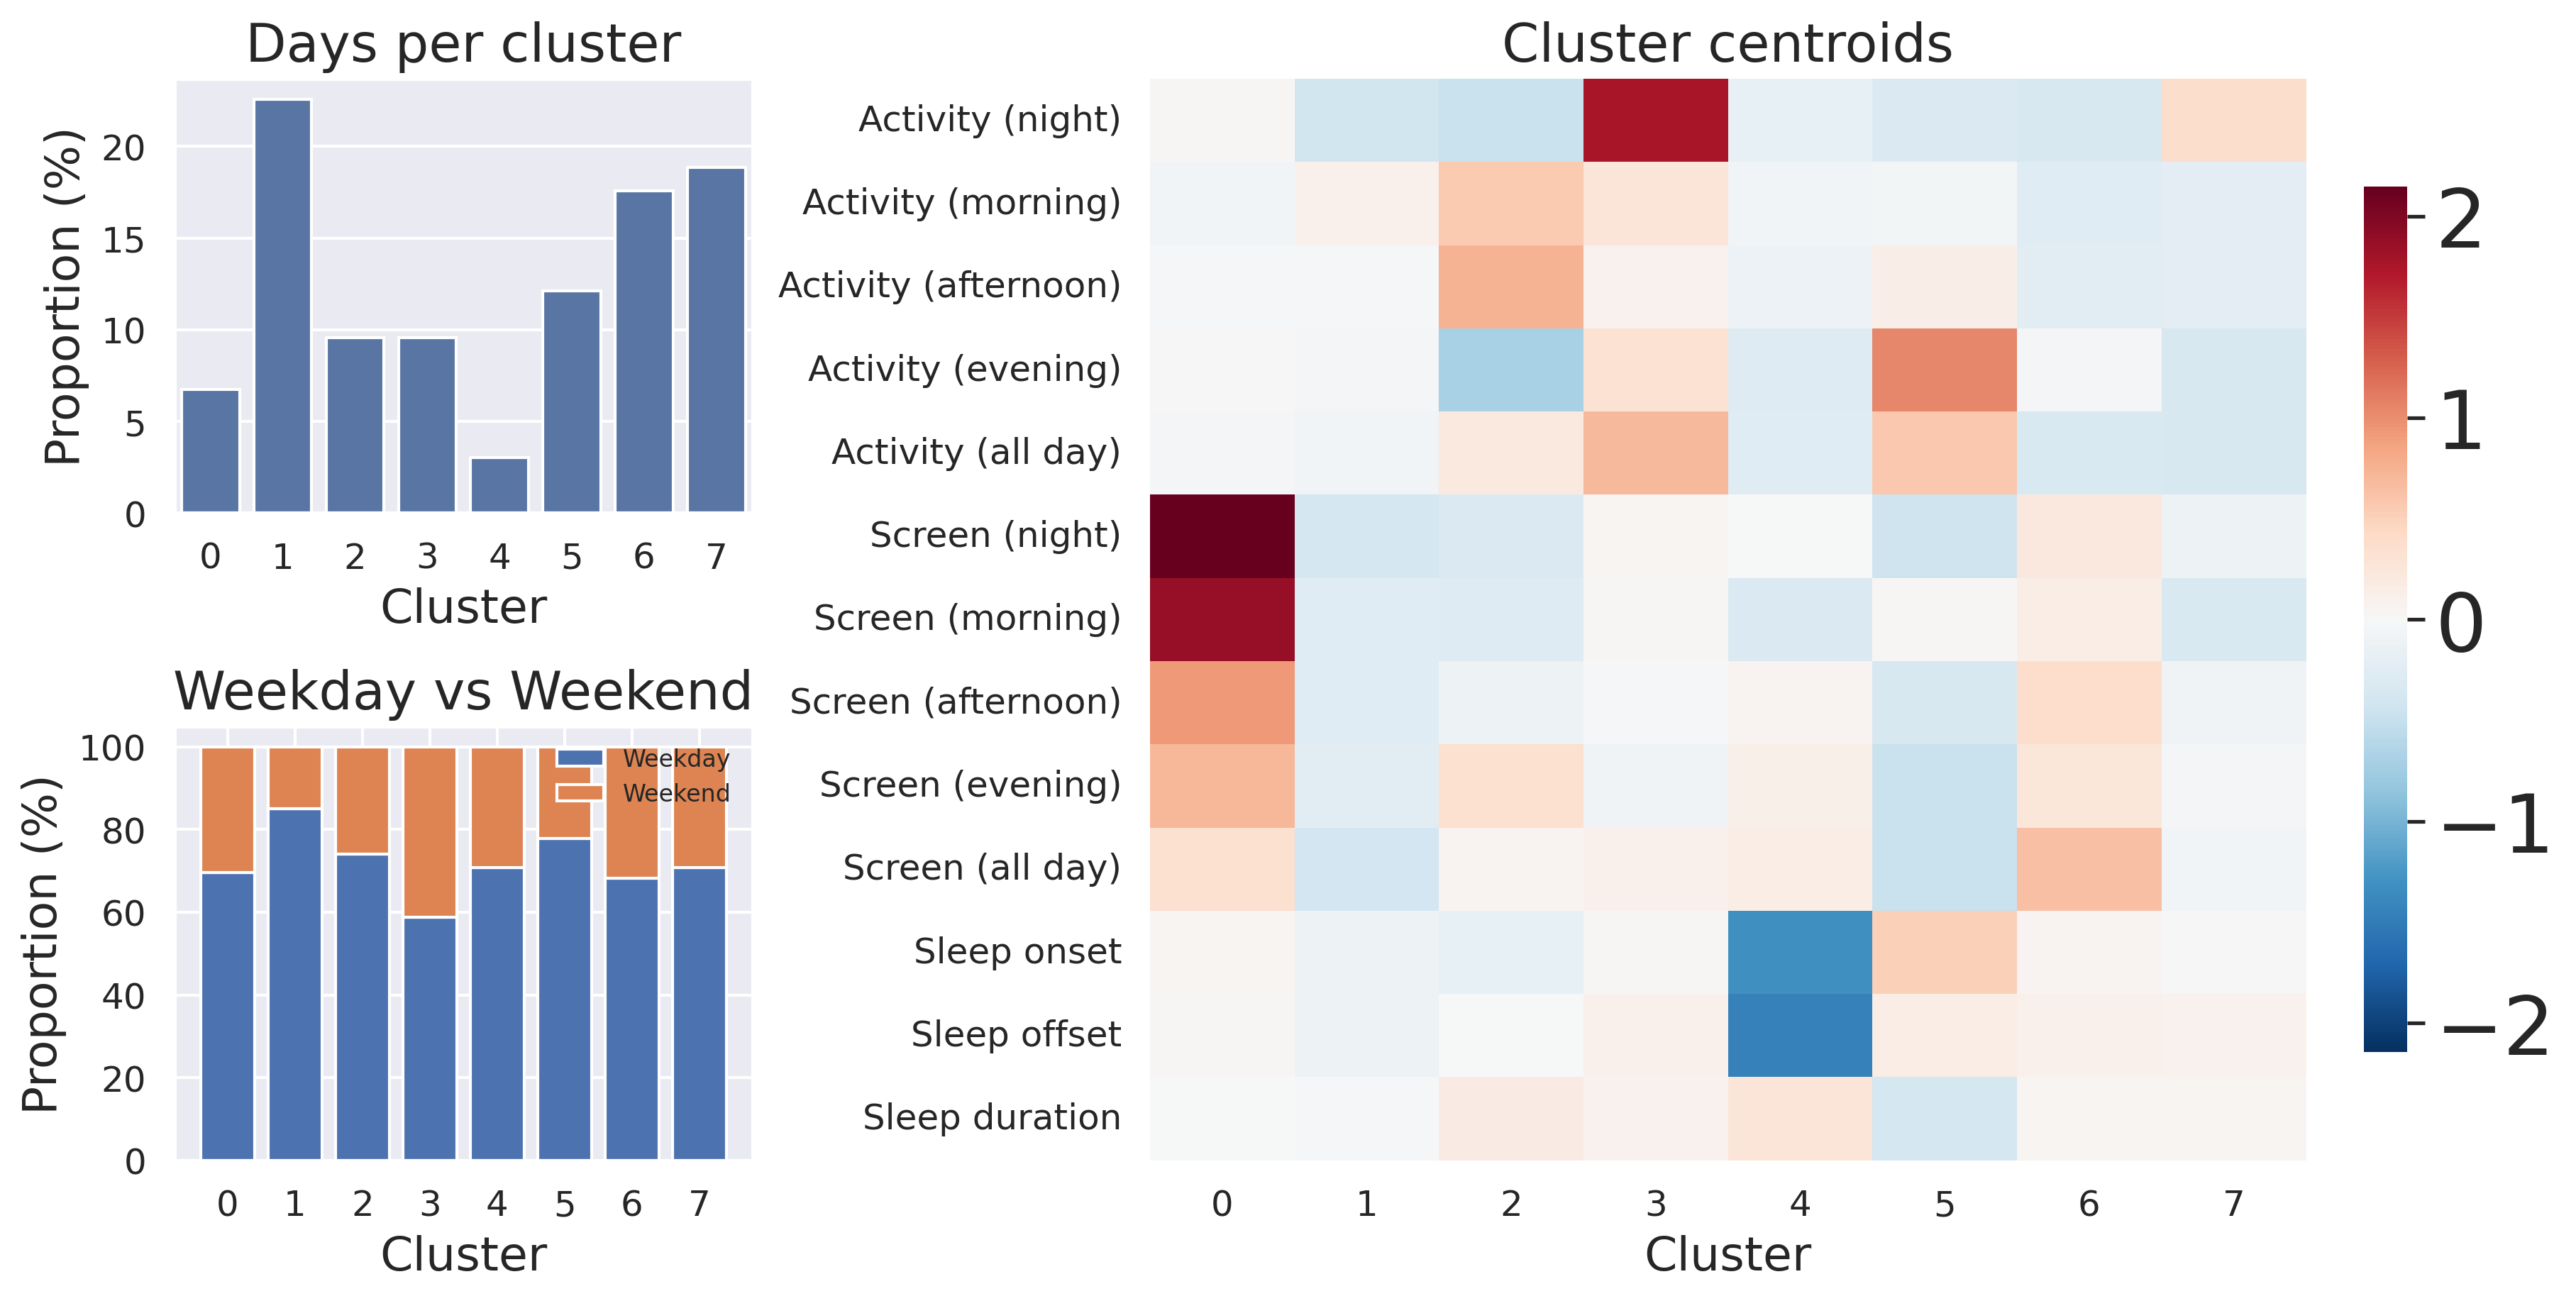
\includegraphics[width=\linewidth]{figures/appendix/globem_INS-W_1_summary.png}
    \caption{Cluster 1}
    \label{fig:globem_centroids_a}
  \end{subfigure}\hfill
  \begin{subfigure}[t]{0.485\textwidth}
    \centering
    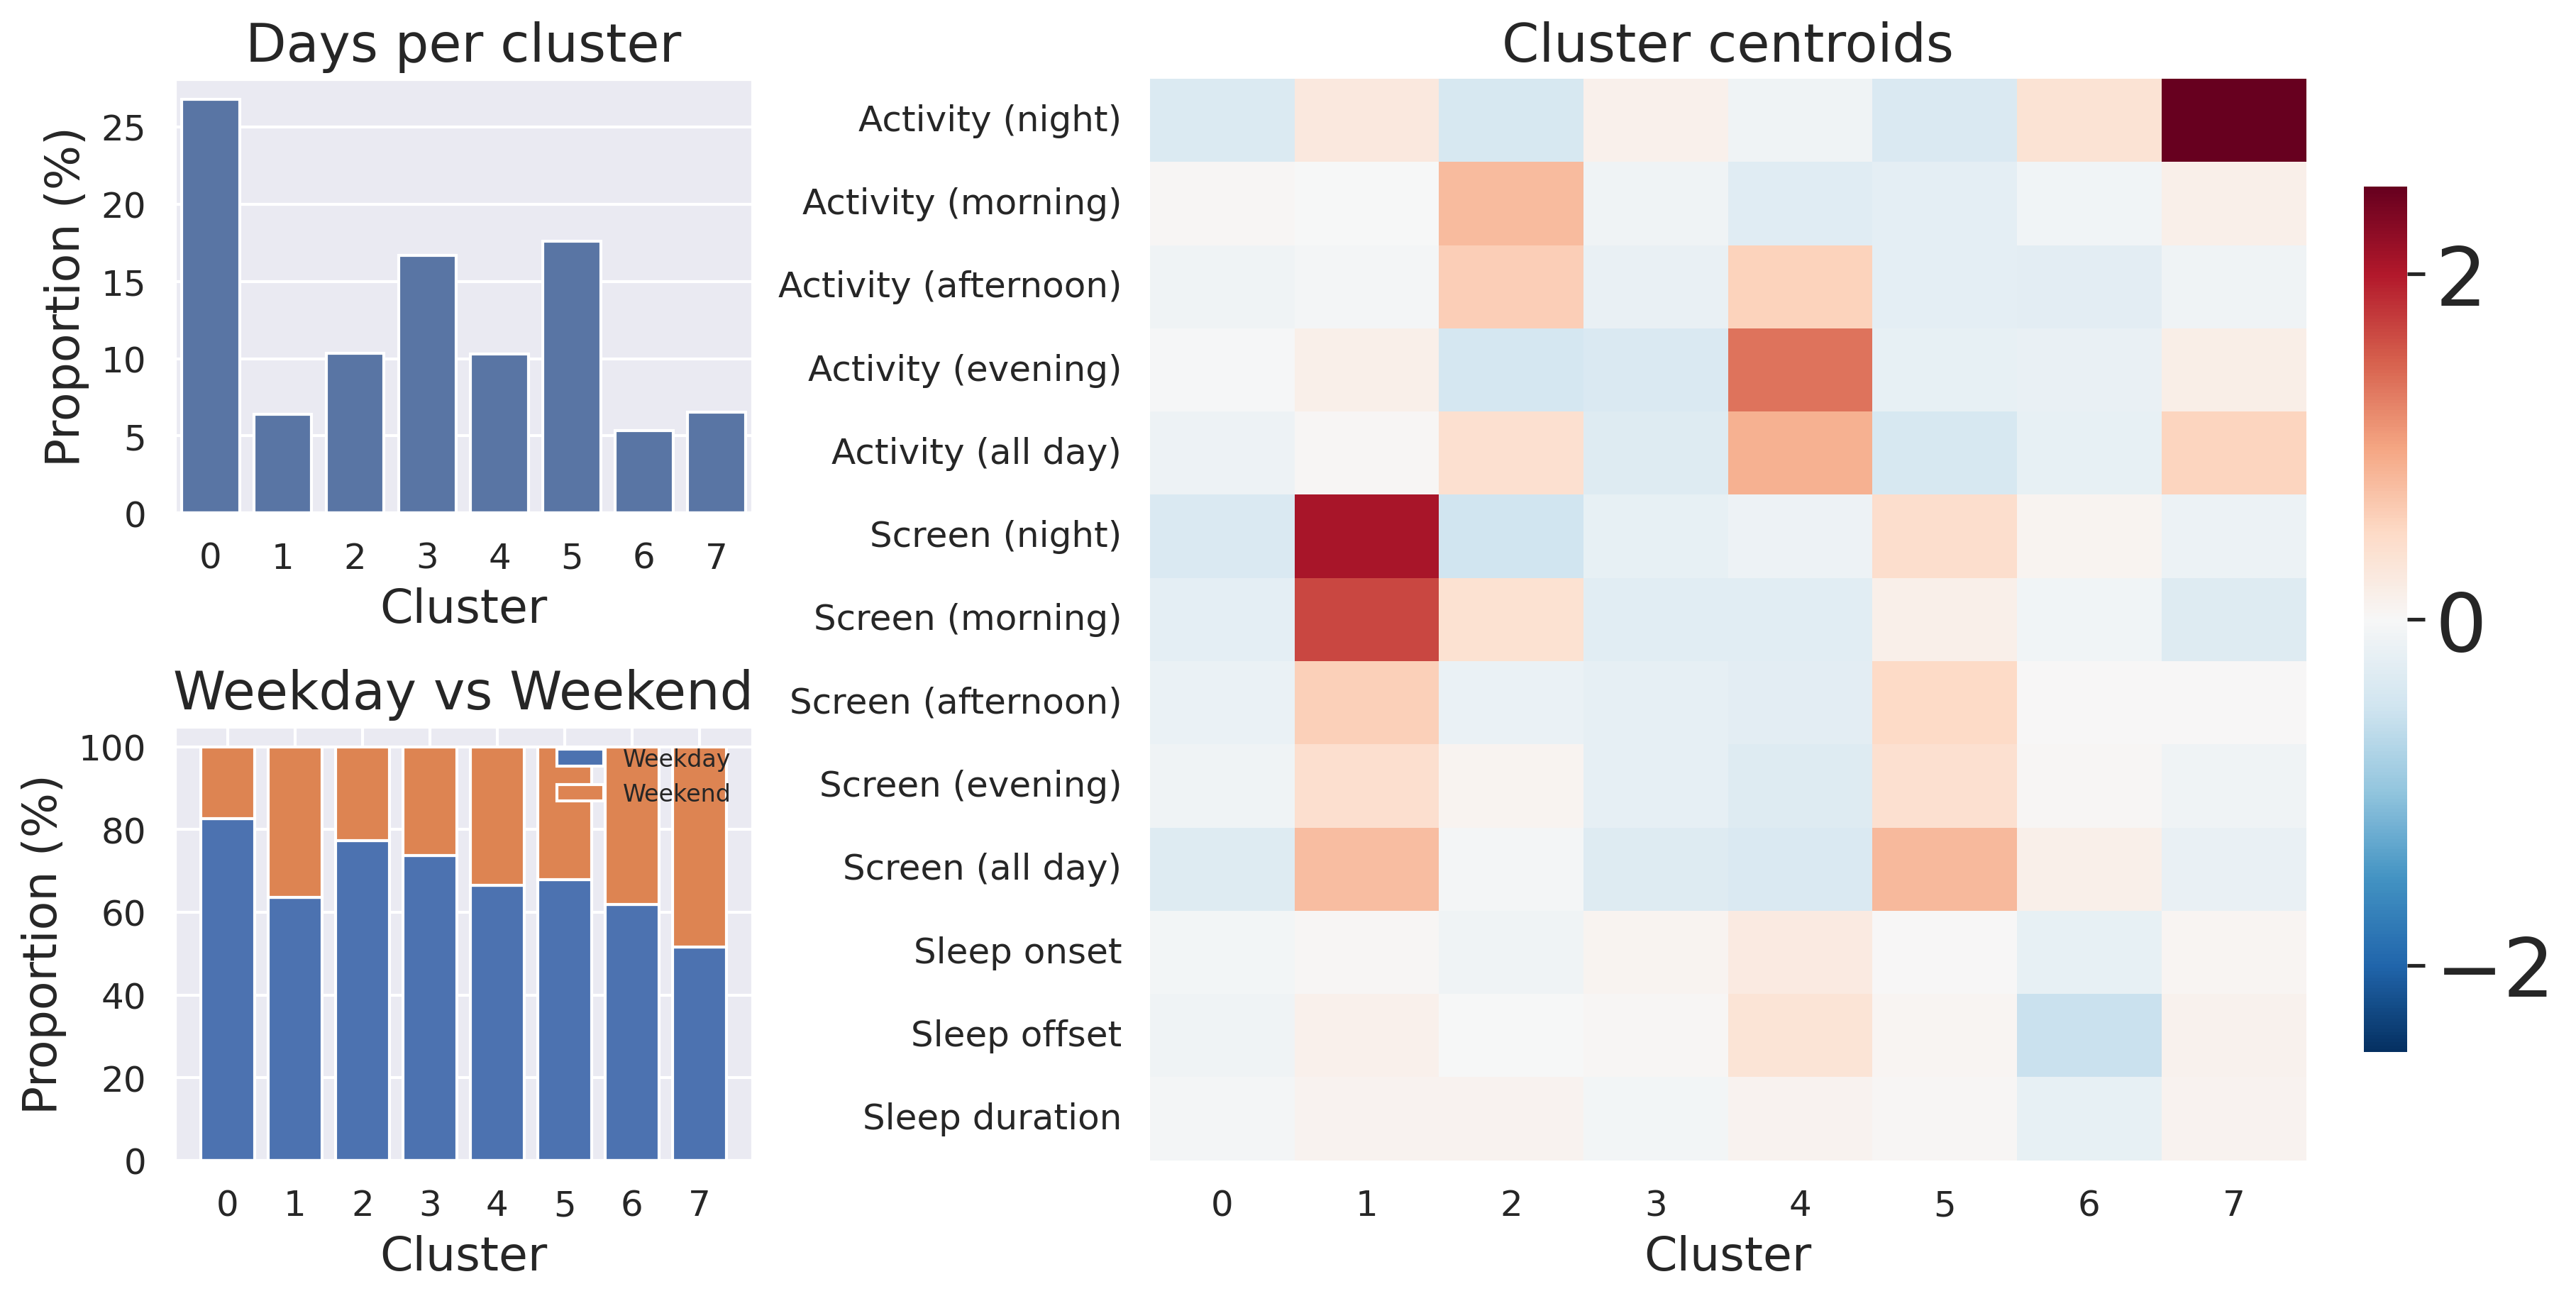
\includegraphics[width=\linewidth]{figures/appendix/globem_INS-W_2_summary.png}
    \caption{Cluster 2}
    \label{fig:globem_centroids_b}
  \end{subfigure}

  \medskip

  \begin{subfigure}[t]{0.485\textwidth}
    \centering
    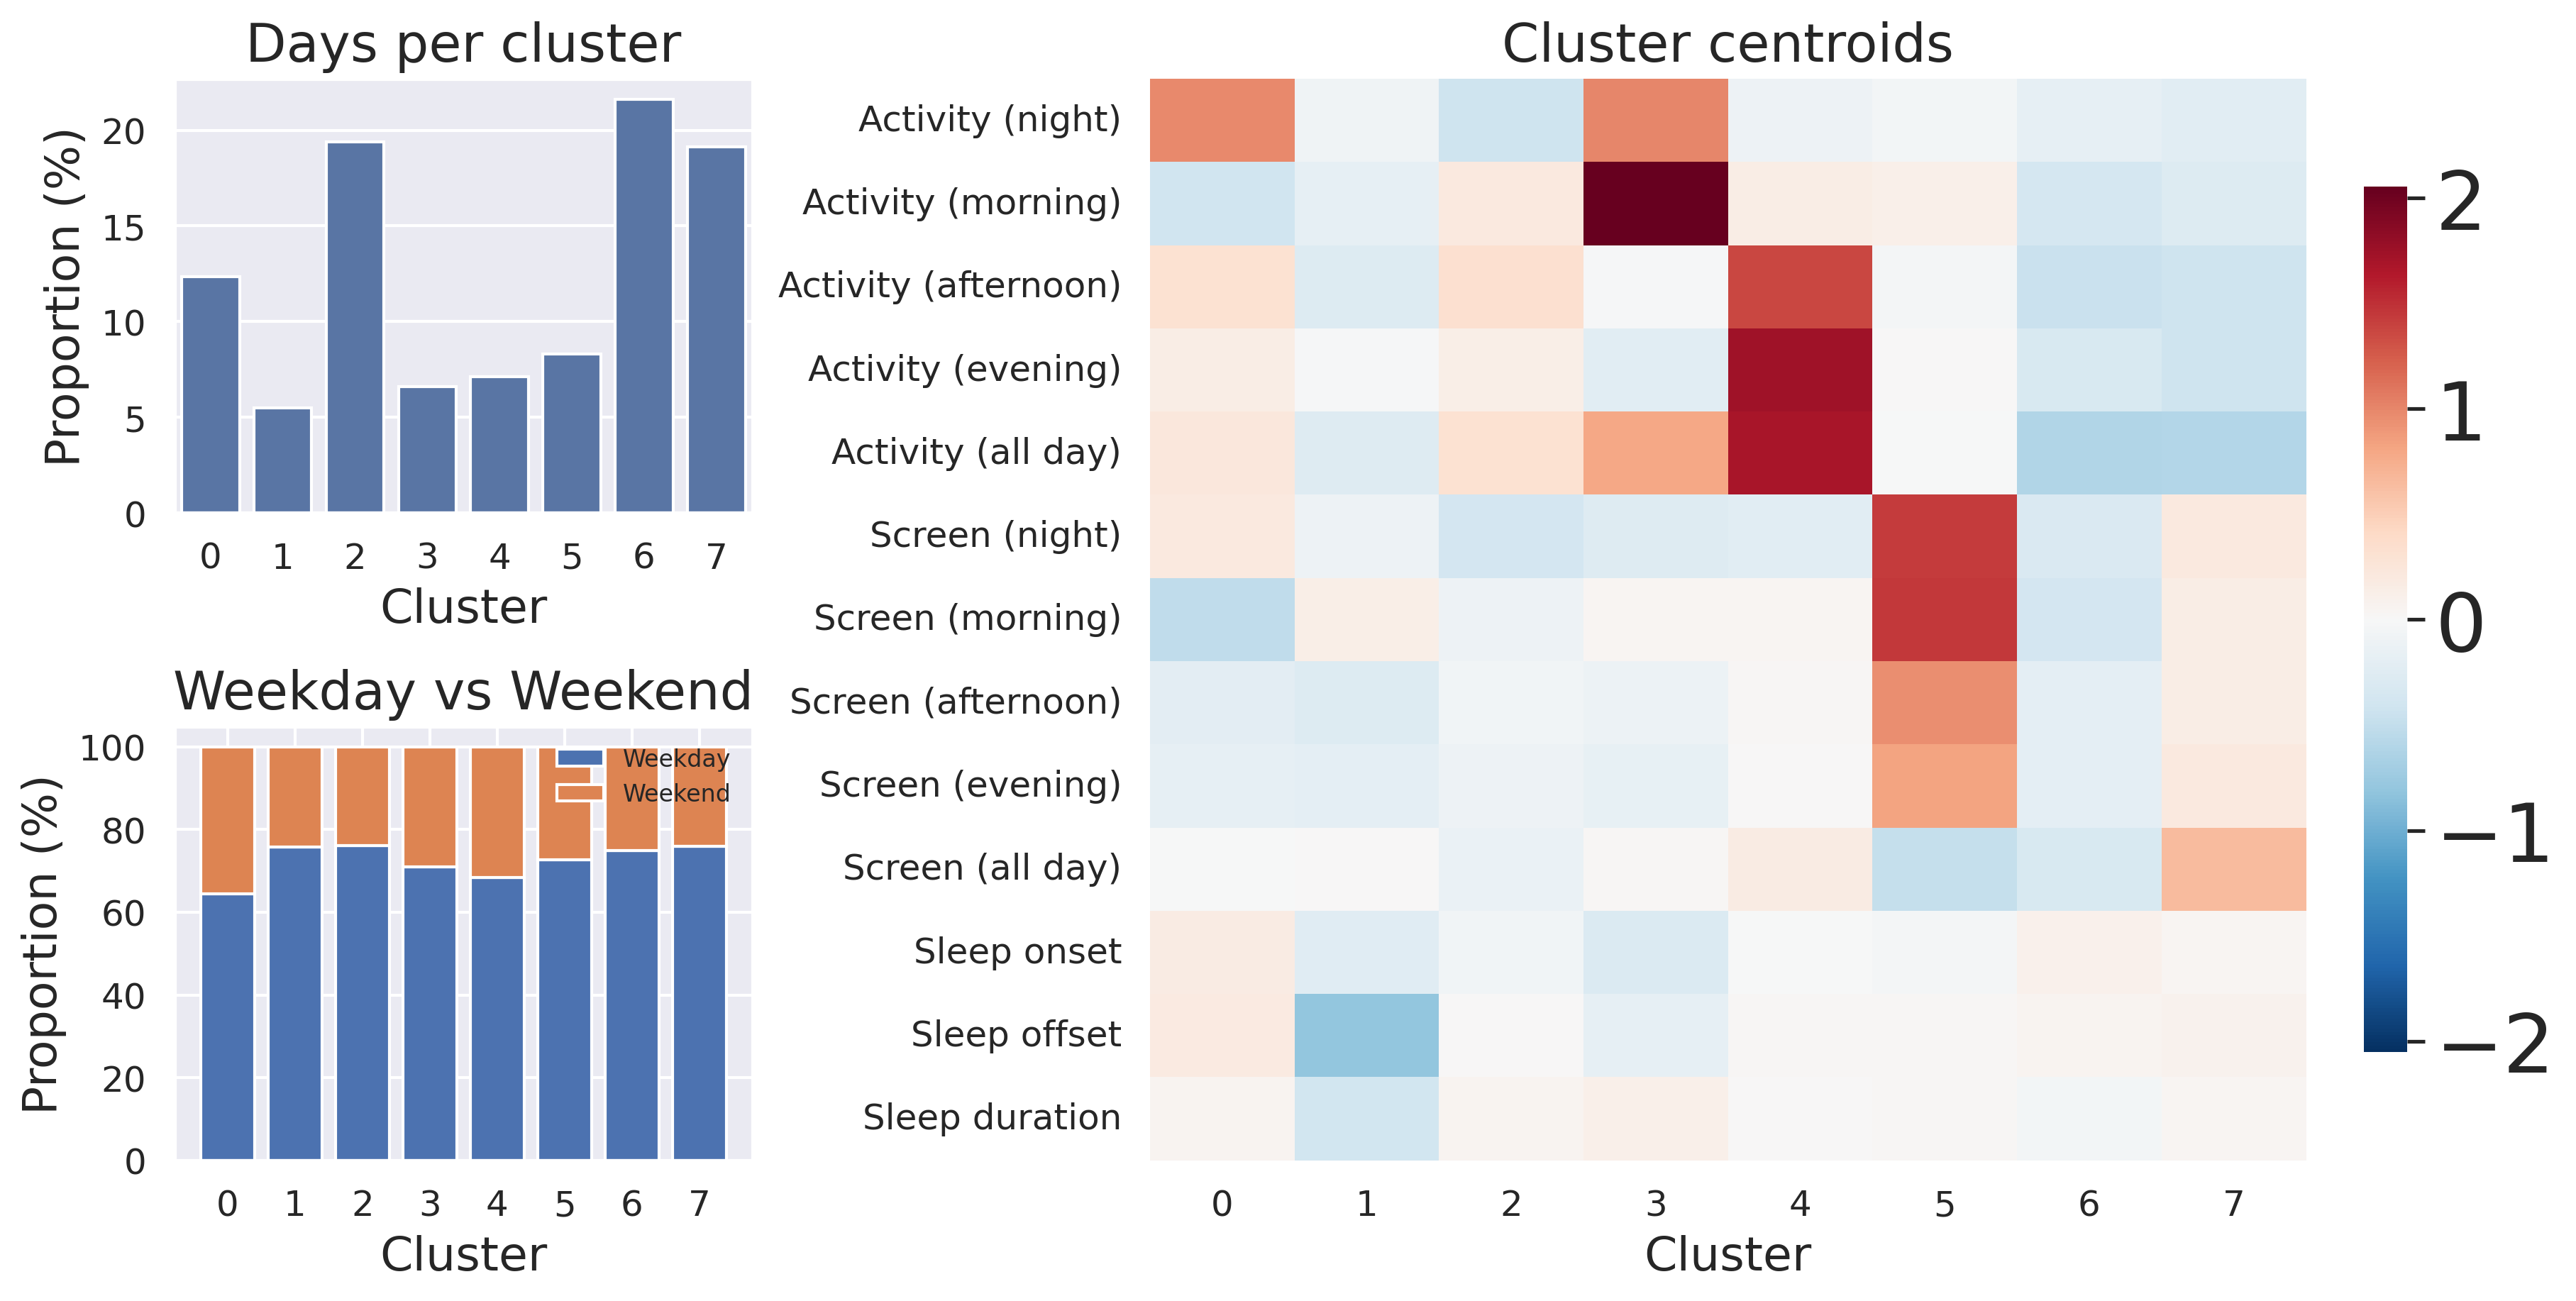
\includegraphics[width=\linewidth]{figures/appendix/globem_INS-W_3_summary.png}
    \caption{Cluster 3}
    \label{fig:globem_centroids_c}
  \end{subfigure}\hfill
  \begin{subfigure}[t]{0.485\textwidth}
    \centering
    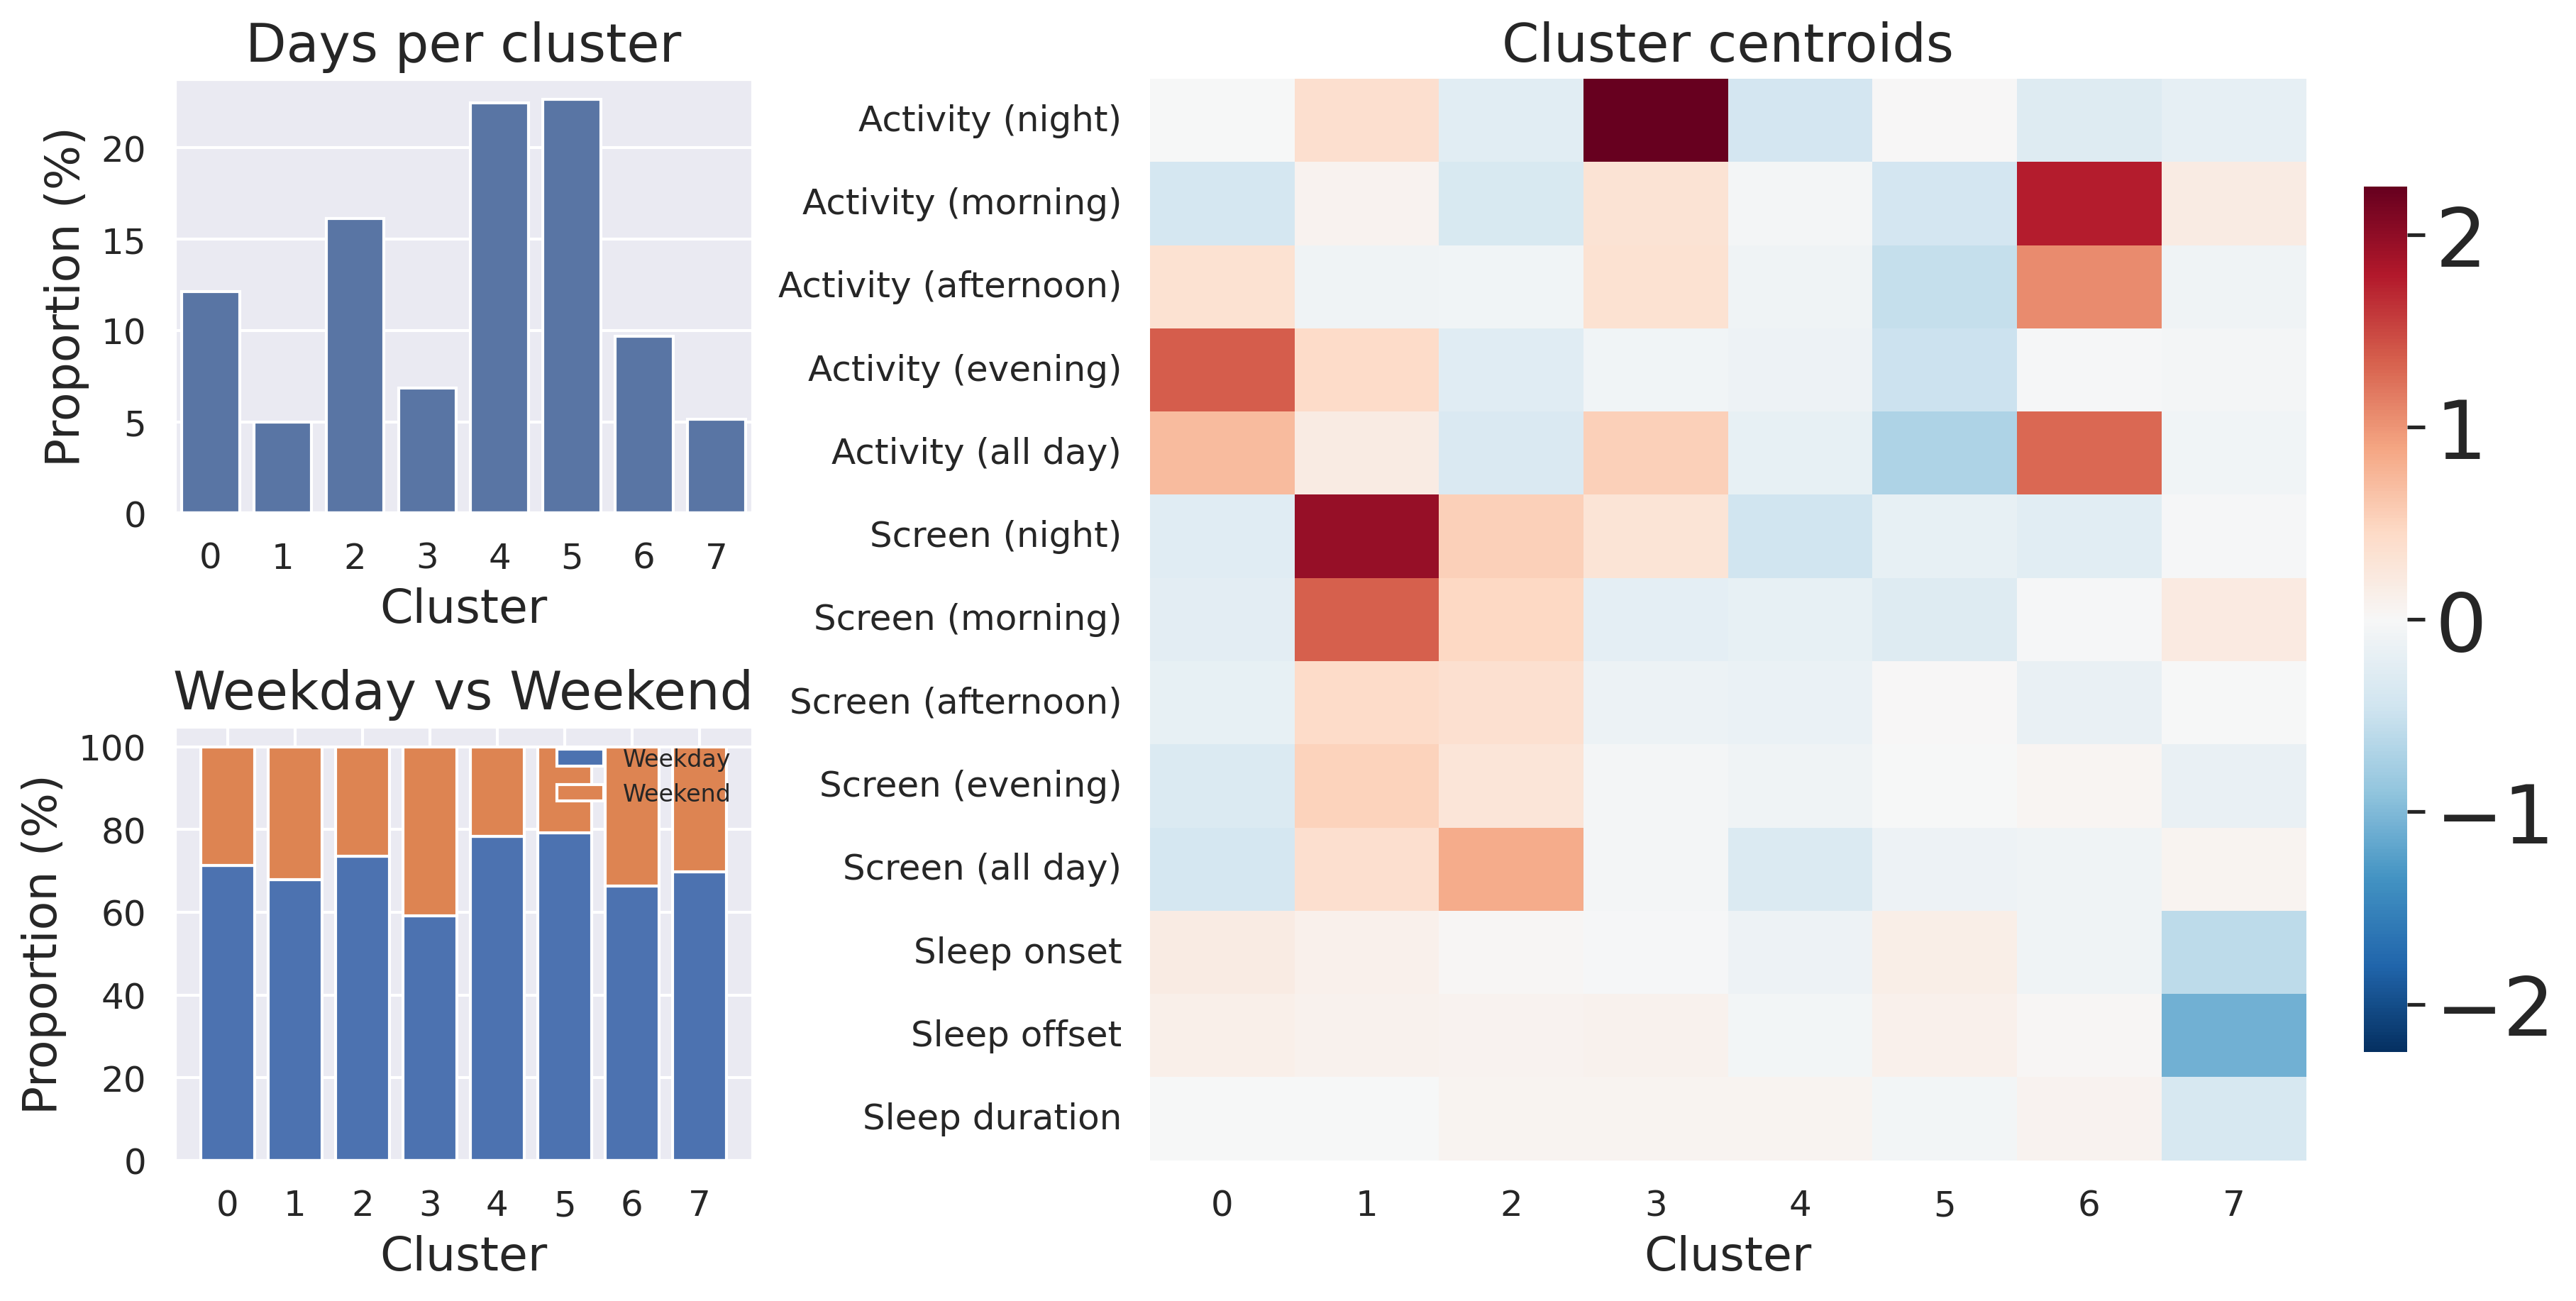
\includegraphics[width=\linewidth]{figures/appendix/globem_INS-W_4_summary.png}
    \caption{Cluster 4}
    \label{fig:globem_centroids_d}
  \end{subfigure}

  \caption{GLOBEM: Cluster centroid characteristics.}
  \label{fig:globem_centroids}
\end{figure}


% ---------- C: Signature with varying K ----------
\clearpage
\section{Signature with varying K components}

% (Add your figures/tables for this section here; using [p] + \FloatBarrier keeps them on this section’s pages.)

% \begin{figure}[p]
%   \centering
%   \includegraphics[width=\linewidth]{figures/appendix/signature_varying_K.png}
%   \caption{Signature stability under varying number of components K.}
%   \label{fig:signature_varying_K}
% \end{figure}
% \FloatBarrier

\end{appendices}
